\chapter{Alternativen}
\label{ch:alt}
Folgendes Kapitel soll die Vor- und Nachteile von möglichen Alternativen zur Datenkommunikation via Bluetooth aufzeigen.

\section{Kabel}
Die simpelste und älteste Methode um Daten auszutauschen ist das Kabel.

\subsubsection{Vorteile}
Alleine durch das Medium ist ein Kabel sicherer als z.B. Funk. Zudem kann die Verbindung verschlüsselt erfolgen, so dass bei langen und nicht übersichtbaren Verbindungen das Abhören massiv erschwert wird.
Kabel sind meist sehr günstig, schnell, stromsparend und es können Standardstecker verwendet werden (z.B. \gls{usbLabel}).

\subsubsection{Nachteile}
Die grössten Nachteile eines Kabels liegen hauptsächlich im Bereich Mobilität.
Zu verwendende Kabel müssen mitgetragen und eingesteckt werden.
Oft erzwingen verschiedene Schnittstellen zudem noch zusätzliche Hardware (weitere Kabel und Adapters), um alle Anforderungen abzudecken.
Für Präsentationen ausserorts, müssen oft mehrere Adapter zur Verfügung stehen, um sicher zustellen, dass alles reibungslos funktioniert.
Diese Vielfalt von Hardware wirkt sich natürlich auch finanziell aus. Zu all dem hängen jeweilige Geräte direkt am Kommunikationspartner, was beispielsweise bei der Nutzung eines Smartphone kaum vorstellbar wäre.

Die genannten Nachteile des Kabels stellten ursprünglich die Motivation für die Möglichkeit einer drahtlosen Kommunikation dar.

\section{Drahtlose Kommunikation}

Mit \textit{drahtloser Kommunikation} wird der Teil einer Verbindung bezeichnet, der oft über elektromagnetischen Wellen (Funk) realisiert wird.
Gerade im Bereich des Internets werden oft nur Endgeräte via Funk angebunden, der Grossteil des Netzes erfolgt aus Kostengründen und Effizienz mit Kabel.

%http://dminc.com/blog/bluetooth-beacons-vs-wifi-vs-nfc/
%https://www.themobilestore.in/blog/bluetooth-vs-nfc-vs-wi-fi-direct/
%http://www.shoppertrak.mx/blog/wifi-bluetooth-ble-nfc-for-retail-marketing/
%http://www.digikey.com/en/articles/techzone/2011/aug/comparing-low-power-wireless-technologies
%https://www.phonegurureviews.com/bluetooth-nfc-wifi-direct/
%http://mobileworldcapital.com/239/



\subsection{Infrarot}
\gls{irLabel} gehörte zu den ersten verbreiteten Möglichkeiten Daten drahtlos zu übermitteln.
1993 gründeten circa 50 Unternehmen die \gls{irdaLabel}, welche die Standardisierung von \gls{irLabel} etablierte.
Mit \gls{irLabel} können Daten bis zu einem Gbit/s (\textit{Giga-IR}) übertragen werden.\footcite{Infrared_Data_Association_Wikipedia_2015-05-22}

\subsubsection{Nachteile}
Die Nachteile von \gls{irLabel} sind Kompatibilitätseinschränkungen und die verminderte Anwendungsabdeckung.
Das Hauptproblem ist die sogenannte \gls{losLabel} Verbindung, bei der sich beide Geräte direkt sehen müssen.
Die Reichweite ist oft auf einen Meter (bei \textit{Giga-IR} sogar auf 10\,cm) beschränkt, wobei im alltäglichen Gebrauch der direkte Sichtkontakt die Reichweite etwa gleichermassen beeinträchtigt (da das Gerät richtig platziert werden muss, was sinnbildlich einem unsichtbaren Kabel entspricht).
\gls{irLabel} liefert zu dem eine eher schlechte Power Effizienz (Power pro Bit), verglichen mit anderen drahtlosen Übermittlungen.\footcite{Comparing_Low_Power_Wireless_Technologies_DigiKey_2015-05-22}


\subsection{Wireless LAN / Wi-Fi Direct - IEEE 802.11}
\textit{\gls{wlanLabel}} (\gls{ieeeLabel} 802.11) und \textit{Wi-Fi Direct} unterscheiden sich darin, dass bei einem gewöhnlichem \gls{wlanLabel} die ganze Kommunikation von einem \gls{apLabel} gesteuert wird, über den meist auch der ganze Datenfluss fliesst. Dies wirkt sich selbst unter optimalen Umständen negativ auf die Übertragungsgeschwindigkeit aus.
Wi-Fi Direct erlaubt eine direkte Kommunikation, zwischen zwei Geräten, ohne \gls{apLabel}.

\subsubsection{Vorteile}
Grundsätzlich gilt das \gls{wlanLabel} als weitverbreitetes und als sehr schnelle Möglichkeit um Daten auszutauschen. Die Reichweite ist mit circa 100\,m relativ weit, was eine angenehme und freie Nutzung ermöglicht.
Zudem ist \gls{wlanLabel} relativ günstig.

\subsubsection{Nachteile}
Eine hohe Geschwindigkeit über Funk, heisst auch einen hohen Stromverbrauch. Wi-Fi Direct noch nicht so lange bekannt wie \gls{wlanLabel}, und wird daher weniger unterstützt.

\subsubsection{Testergebnisse}
Um die effektive Geschwindigkeit zu messen wurden mehrere Versuche durchgeführt.
Dabei sendete ein Android Gerät (Oneplus One) Daten an ein Macbook Air (13 Zoll, Early 2014, mit einem AirPort Extreme Wi-Fi Adapter).
Das Android Gerät stellte die Daten mit Hilfe von SuperBeam\footcite{SuperBeam_WiFi_Direct_Share_Android_Apps_on_Google_Play_2015-05-22} (einer Android App) zur Verfügung.

Dabei wurden folgende Schritte durchgeführt
\begin{itemize}
	\item Die Datei wird auf Smartphone ausgewählt.
	\item SuperBeam stellt ein Wi-Fi Direct Netz auf, an dem sich der Empfänger anmelden kann. Falls das Smartphone bereits mit einem \gls{wlanLabel} verbunden ist, bietet es die Option über das bestehende Netzwerk die Daten auszutauschen.
	Das Smartphone kann immer nur eine Wi-Fi Verbindung aufrecht halten, das heisst wird Wi-Fi Direct genutzt, müssen beidseitig andere Wireless-Verbindungen unterbrochen werden.
	\item Die Datei kann via einer URL heruntergeladen werden.
\end{itemize}

\begin{figure}[H]
	\centering
	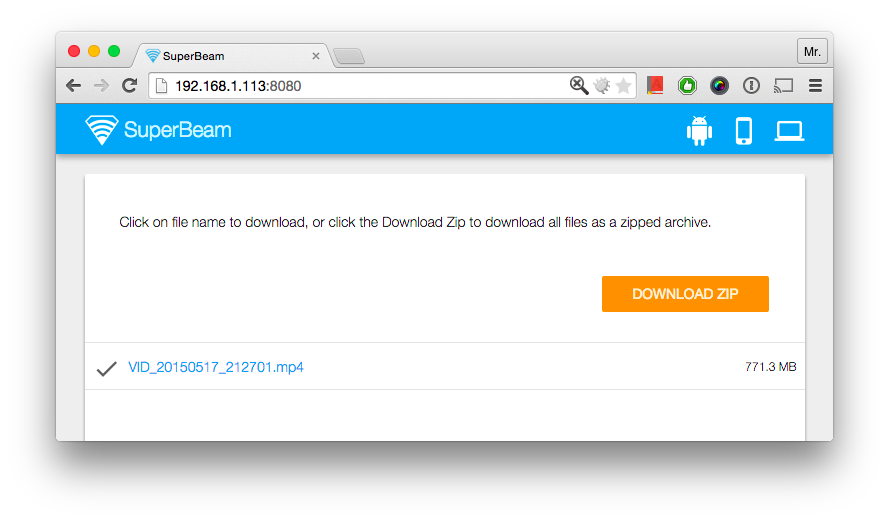
\includegraphics[width=0.9\textwidth]{images/alternatives/superbeam_web.png}
	\caption{SuperBeam Web-Frontend Ansicht}
\end{figure}

Bei den Tests wurden folgende Übertragungsgeschwindigkeiten gemessen (Filetransfer von $\approx770$\,MB):
\begin{table}[H]
	% style
	\small\sffamily\renewcommand{\arraystretch}{1.4}
	% caption
	\captionabove{\gls{wlanLabel} vs. Wi-Fi Direct}
	\begin{tabular}{lp{0.35\linewidth}p{0.30\linewidth}}
		\toprule
		Technologie & Bit & Byte\\
		\midrule
		\gls{wlanLabel} & 0.8 - 6.4 Mbit/s & 0.1 - 0.8\,MB/s\\
		Wi-Fi Direct & 46\,Mbit/s & 5.75\,MB/s\\
		\bottomrule
	\end{tabular}
\end{table}

Besonders auffallend sind die bleibenden Schwankungen bei der \gls{wlanLabel} Übertragung.
Obwohl das Netzwerk nebst des Datentransfers kaum belastet wurde, variiert die Geschwindigkeit dauernd (bis um das Achtfache des Minimums).
Selbstverständlich spielt die Distanz und die Abschottung zwischen \gls{apLabel} und Client eine erhebliche Rolle, die wurde jedoch nach dem ersten Test minimiert, indem beide Geräte direkt neben dem \gls{apLabel} gelegt wurden.

Beim Wi-Fi Direct hat sich die Geschwindigkeit sehr rasch bei 46\,Mbit/s stabilisiert, was gegenüber der Verbindung mit dem \gls{apLabel} (mit durchschnittlich 3.6\,Mbit/s) eine über zwölffache schnellere Geschwindigkeit ermöglicht.
Dies reduziert die Wartezeit mit Wi-Fi Direct auf beinahe 8\,\%.

\subsection{NFC}
\gls{nfcLabel} ist seit 2002 spezifiziert und wurde 2006 erstmalig in einem Smartphone eingebaut.
Die Technologie erlaubt innerhalb von 10\,cm eine Datenübertragung von max. 424\,kbit/s.
Je nach Anwendungsfall kann die Reichweite auf einen Meter erweitert werden, wozu allerdings eine 1.5\,m hohe Antenne benötigt wird (dies kann z.B. in einem Warenhaus vorkommen).\footcite{Near_Field_Communication_Wikipedia_2015-05-22}

Die Technologie kann vor allem für bargeldloses Zahlen verwendet werden.
Aufgrund der tiefen Übertragungsrate eignet sich \gls{ncfLabel} nicht besonders für den Austausch von gewöhnlichen Dateien (Bilder, Dokumente, etc.).
Zudem darf während der Übertragungen die maximale Reichweite nicht überschritten werden, was die Handhabung nicht unbedingt bequem machen muss.
Sofern kleine Datenmengen (vor allem textbasierte Daten) wie Kontakte, Links oder Einstellungen übertragen werden sollen, kann \gls{nfcLabel} genutzt werden. Allerdings ist eine Kommunikation zwischen verschiedenen Systemen oft nicht möglich, weil die Programmen keine einheitlichen Schnittstellen anbieten.

\subsubsection{Vorteile}
Durch die stark beschränkte Reichweite, wird unerlaubter Zugriff praktisch verunmöglicht.
Die Nutzung ist sehr einfach gehalten, es reicht der Kontakt der Geräten um Daten auszutauschen ("`\textit{beamen}"').
Die Technologie bietet sich für sicherheitsrelevante Übertragungen von kleinen Datenmengen an.
Einzelne \gls{rfidLabel}'s, die eine Identifizierung ermöglichen, können sehr günstig erworben werden.

\subsubsection{Nachteile}
\gls{nfcLabel} wurde als eigene Technologie zum existierenden Bluetooth und \gls{wlanLabel} entwickelt. Dabei wurde bewusst ein eigener Anwendungsbereich anvisiert. Also ist die tiefe Datenübertragungsrate und die kurze Reichweite eine gewollte Funktion und kein Nachteil.
Hingegen handelt es sich bei \gls{nfcLabel} um eine zertifizierte Technologie.
Gerade im Zusammenhang mit der raren Verbreitung, stellt diese Zertifizierung eine grosse Hürde für das Angebot von dieser Technologie dar.

% http://www.mobilepaymentstoday.com/blogs/ble-vs-nfc-the-future-of-mobile-consumer-engagement-now-infographic/


% \subsection{Bluetooth}

